\begin{figure}[H]
\centering
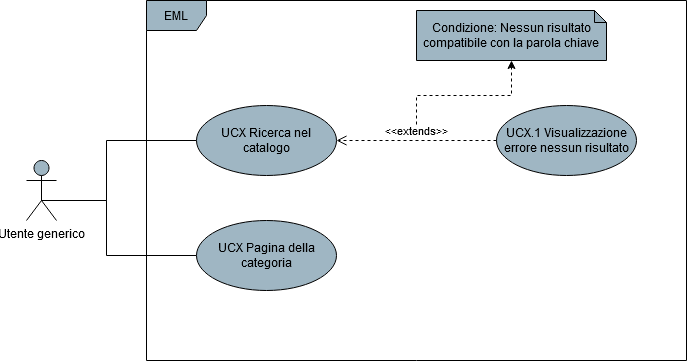
\includegraphics[scale=0.6]{res/UseCase/Immagini/NavigazioneCatalogoGenerale}
\caption{Schema generale: modulo di navigazione del catalogo}
\end{figure}
\subsubsection{UC10 - Ricerca nel catalogo digitale}
\begin{itemize}
\item \textbf{Attori primari}: utente generico;
\item \textbf{Descrizione}: l'utente può effettuare una ricerca tra tutti i prodotti in vendita nella piattaforma attraverso la digitazione di una parola o frase chiave nella barra di ricerca;
\item \textbf{Scenario Principale}: l'utente seleziona la barra di ricerca e inserisce la parola chiave corrispondente al prodotto desiderato. Infine se la ricerca va a buon fine viene visualizzata una lista di prodotti compatibili con la parola digitata, altrimenti viene visualizzato un messaggio che informa che la ricerca non ha prodotto nessun risultato;
\item \textbf{Precondizione}: l'utente si trova sulla piattaforma e necessita di fare una ricerca per trovare un prodotto specifico;
\item \textbf{Postcondizione}: l'utente visualizza il risultato della ricerca effettuata.
\end{itemize}
\subsubsection{UC11 - Accesso ad una pagina della categoria}
\begin{itemize}
\item \textbf{Attori primari}: utente generico;
\item \textbf{Descrizione}: l'utente può accedere ad una pagina contenente un insieme di prodotti listati facenti parte di una specifica categoria. In questa pagina, chiamata anche PLP\ped{G}, l'utente ha a disposizione ulteriori strumenti per interagire con i prodotti da lui desiderati [\textbf{UC12}];
\item \textbf{Scenario Principale}: l'utente clicca sulla categoria di prodotti da lui desiderata.
\item \textbf{Precondizione}: l'utente si trova sulla piattaforma e necessita di visualizzare tutti i prodotti contenuti in una specifica categoria;
\item \textbf{Postcondizione}: l'utente accede alla PLP\ped{G} corrispondente alla categoria desiderata.
\end{itemize}
\begin{figure}[H]
\centering
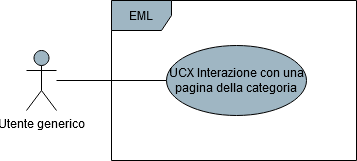
\includegraphics[scale=0.6]{res/UseCase/Immagini/InterazionePaginaCategoriaGenerale}
\caption{Schema generale: modulo di interazione con una pagina di categoria}
\end{figure}